\section{Filtros, Limpieza y Transformaciones Finales}
\label{sec:limpieza_transformacion}

De acuerdo con los requisitos de la entrega final, una vez consolidado el entendimiento del negocio y de los datos, se culminó el pipeline de limpieza, filtrado y transformación distribuida en \textbf{Apache Spark} (\texttt{spark://10.195.34.34:7077}). El diseño se estructuró en tres capas de datos en memoria: (i) \textit{datos de origen} (\texttt{df\_arrests}, \texttt{df\_col\_raw}, \texttt{df\_poverty}), que preservan los registros recibidos para auditar esquemas y nulos; (ii) \textit{datos depurados} (\texttt{arr\_dep}, \texttt{col\_dep}, \texttt{pov\_dep}), sobre los cuales se aplican las reglas de filtrado de integridad; y (iii) \textit{datos para análisis y modelado} (\texttt{arr\_analisis}, \texttt{col\_analisis}, \texttt{pov\_analisis}), enriquecidos con las transformaciones e imputaciones requeridas para responder las preguntas de negocio y entrenar los modelos en \textbf{Spark MLlib}.

\subsection{Filtros Aplicados y su Justificación Técnica y de Negocio}
\label{subsec:filtros_inconsistentes}

Se implementaron \textbf{cuatro filtros principales} sobre los DataFrames de Spark (superando el mínimo de dos filtros exigido), complementados con un filtro lógico no destructivo para coordenadas geoespaciales (\texttt{coord\_valida}). La Tabla \ref{tab:reglas_filtrado} detalla cada regla y su justificación.

\begin{table}[H]
\centering
\scriptsize
\renewcommand{\arraystretch}{1.25}
\caption{Reglas finales de filtrado implementadas en PySpark y su justificación.}
\label{tab:reglas_filtrado}
\begin{tabularx}{\linewidth}{c l >{\raggedright\arraybackslash}p{3.6cm} >{\raggedright\arraybackslash}p{4.2cm} X}
\toprule
\textbf{\#} & \textbf{Dataset} & \textbf{Problema detectado} & \textbf{Filtro aplicado en PySpark} & \textbf{Justificación técnica y de negocio} \\
\midrule
F1 & Collisions & Filas desplazadas por saltos de línea, llave ausente o conteos no convertibles / negativos en las 8 columnas \texttt{NUMBER OF...} & Lectura con \texttt{multiLine=True}, \texttt{quote}, \texttt{escape}; \texttt{COLLISION\_ID.isNotNull() \& length > 0} y \texttt{try\_cast(c AS INT) >= 0} en las 8 columnas de víctimas. & Garantiza que cada registro represente un evento vial real y elimina corrupciones de parseo (p.\,ej., el valor espurio de $3,291,249$ en ciclistas heridos detectado en el EDA). \\
F2 & Collisions & Incoherencia aritmética entre subcategorías y el total de víctimas del choque & \texttt{(PEDESTRIANS + CYCLIST + MOTORIST INJURED) <= PERSONS INJURED} (e idéntica condición para \texttt{KILLED}). & Peatones, ciclistas y motoristas son subconjuntos disjuntos del total de personas afectadas; violar esta desigualdad altera las tasas de letalidad de \textit{Vision Zero}. \\
F3 & Collisions \& Arrests & Duplicidad de registros de eventos por llave primaria & \texttt{dropDuplicates(['COLLISION\_ID'])} en colisiones y \texttt{ARREST\_KEY.isNotNull()} con \texttt{dropDuplicates(['ARREST\_KEY'])} en arrestos. & Previene el doble conteo de detenciones o siniestros viales en las agregaciones territoriales y en el entrenamiento supervisado. \\
F4 & Poverty & Factores de expansión muestral nulos o no positivos & \texttt{filter(F.col('PWGTP') > 0)} sobre los microdatos socioeconómicos. & Las estimaciones ponderadas de población, pobreza y desempleo exigen pesos muestrales estrictamente positivos como denominador. \\
\bottomrule
\end{tabularx}
\end{table}

\subsubsection{Evidencia Cuantitativa de los Filtros (Conteos Antes y Después)}

La Tabla \ref{tab:conteos_filtros} reporta el resultado exacto de la ejecución distribuida de los filtros F1 a F4 sobre el clúster de Spark, junto con la evaluación del indicador de calidad espacial \texttt{coord\_valida} (definido como $\text{lat} \in [40.49^\circ, 40.92^\circ]$ y $\text{lon} \in [-74.27^\circ, -73.68^\circ]$ en colisiones, y $X \in [900{,}000, 1{,}070{,}000]$, $Y \in [110{,}000, 275{,}000]$ pies NAD 83 en arrestos). Conservar los registros con \texttt{coord\_valida = False} en la tabla general y filtrarlos únicamente en las consultas geoespaciales evita perder información válida en los análisis temporales y categóricos.

\begin{table}[H]
\centering
\scriptsize
\renewcommand{\arraystretch}{1.2}
\caption{Conteo de registros antes y después de los filtros de integridad y validación espacial en Spark.}
\label{tab:conteos_filtros}
\resizebox{\textwidth}{!}{%
\begin{tabular}{l r r r r r}
\toprule
\textbf{Conjunto de Datos} & \textbf{Registros antes} & \textbf{Registros después} & \textbf{Descartados} & \textbf{\texttt{coord\_valida = True}} & \textbf{\texttt{coord\_valida = False}} \\
\midrule
NYPD Arrest Data & 141,870 & 141,870 & 0 & 141,861 (99.99\%) & 9 (0.01\%) \\
Motor Vehicle Collisions & 2,305,623 & 2,305,355 & 268 & 2,056,013 (89.18\%) & 249,342 (10.82\%) \\
NYCgov Poverty Measure & 68,273 & 68,273 & 0 & N/A (nivel \texttt{Boro}) & N/A \\
\bottomrule
\end{tabular}%
}
\end{table}

\subsection{Transformaciones Finales y su Justificación}
\label{subsec:limpieza_datos}

Sobre los datos depurados se aplicaron \textbf{seis transformaciones distribuidas} (superando ampliamente el mínimo de tres transformaciones requerido), resumidas en la Tabla \ref{tab:transformaciones_finales}.

\begin{table}[H]
\centering
\scriptsize
\renewcommand{\arraystretch}{1.25}
\caption{Transformaciones finales implementadas sobre los DataFrames en Apache Spark.}
\label{tab:transformaciones_finales}
\begin{tabularx}{\linewidth}{c l >{\raggedright\arraybackslash}p{4.3cm} X}
\toprule
\textbf{\#} & \textbf{Dataset} & \textbf{Transformación implementada} & \textbf{Justificación técnica y de negocio} \\
\midrule
T1 & Todos & \textbf{Conversión de separadores numéricos y tipos:} Reemplazo de coma decimal por punto en coordenadas (\texttt{replace(LATITUDE, ',', '.')}) y limpieza de puntos de miles y comas decimales en las $22$ columnas monetarias de pobreza (\texttt{EST\_*}, \texttt{*\_adj}, \texttt{NYCgov\_Income}, \texttt{NYCgov\_Threshold}, \texttt{PreTaxIncome\_PU}) antes de aplicar \texttt{try\_cast(... AS DOUBLE)}. & Los archivos CSV utilizan convención numérica local; sin esta transformación, el motor infiere las coordenadas y los ingresos como texto (\texttt{StringType}) o produce \texttt{NULL} al convertirlos directamente. \\
T2 & Arrests \& Collisions & \textbf{Estandarización temporal y textual:} Conversión de \texttt{ARREST\_DATE} y \texttt{CRASH DATE} a \texttt{DateType} (\texttt{MM/dd/yyyy}), extracción de la hora entera $\texttt{hora} \in \{0,\dots,23\}$ desde \texttt{CRASH TIME} (\texttt{H:mm}), e higienización textual (\texttt{F.upper(F.trim(...))}) en descripciones delictivas, calles, vehículos y factores. & Habilita el particionamiento temporal por año/semestre, el análisis horario de siniestralidad y elimina categorías duplicadas por diferencias de mayúsculas o espacios en blanco. \\
T3 & Arrests & \textbf{Depuración de catálogo e imputación jerárquica de \texttt{LAW\_CAT\_CD} por moda condicionada:} Preservación de la columna original en \texttt{gravedad\_reportada}; recodificación a \texttt{NULL} de valores fuera de \texttt{\{F, M, V\}} (\texttt{'9'}, \texttt{'I'}, \texttt{'(null)'}) e imputación de los $1,394$ nulos mediante la moda de \texttt{LAW\_CAT\_CD} particionada por código interno de delito (\texttt{Window.partitionBy('PD\_CD')}), con respaldo en la moda global (\texttt{M}). & Dado que cada código interno \texttt{PD\_CD} tipifica un delito específico, imputar según la moda de su propio \texttt{PD\_CD} preserva la correspondencia jurídica real (dejando $0$ nulos), mientras que conservar \texttt{gravedad\_reportada} evita alterar los conteos descriptivos de las preguntas 1, 2 y 6. \\
T4 & Collisions \& Poverty & \textbf{Codificación explícita de nulos estructurales:} Asignación de la etiqueta \texttt{SIN\_VEHICULO\_3..5} en los tipos y factores de vehículos 3 a 5 de colisiones, y del código centinela $-1$ en \texttt{ENG}, \texttt{JWTR}, \texttt{WKW}, \texttt{ESR}, \texttt{MSP} y \texttt{LANX} de pobreza, más normalización de \texttt{AGE\_GROUP} fuera de catálogo a \texttt{DESCONOCIDO}. & Distingue la ausencia estructural (choques con menos de 3 vehículos o saltos lógicos del cuestionario censal) de la pérdida accidental de información, logrando $0$ nulos en todas las variables tratadas. \\
T5 & Todos & \textbf{Armonización interinstitucional de condados (\texttt{BORO}) y cálculo de tasas por $100,000$ habitantes:} Homologación de códigos numéricos (\texttt{1..5} en pobreza) y alfabéticos (\texttt{B, K, M, Q, S} en arrestos) al nombre estándar en mayúsculas (\texttt{BRONX, BROOKLYN, MANHATTAN, QUEENS, STATEN ISLAND}) y cálculo de tasas dividiendo por la población expandida $\sum \texttt{PWGTP}$. & Permite cruzar los tres conjuntos de datos y comparar condados de tamaños demográficos muy dispares (desde $469,393$ hab. en Staten Island hasta $2,540,638$ hab. en Brooklyn) bajo una métrica epidemiológica y criminológica estándar. \\
T6 & Collisions \& Arrests & \textbf{Ingeniería de características espaciales y matemáticas para MLlib:} Discretización en cuadrículas de $0.01^\circ \times 0.01^\circ$ ($\texttt{x} = \lfloor \texttt{lon}\times 100\rfloor$, $\texttt{y} = \lfloor \texttt{lat}\times 100\rfloor$), codificación cíclica de la hora ($\sin(2\pi h/24)$, $\cos(2\pi h/24)$), transformación logarítmica $\log(1+x)$ de conteos por zona e indicadores binarios de fatalidad y afectación a vulnerables. & Provee las variables de entrada estandarizadas para el ranking espacial (Pregunta 5), la Regresión Logística, el agrupamiento K-Means y la Red Neuronal Profunda. \\
\bottomrule
\end{tabularx}
\end{table}

\subsubsection{Resultados de la Transformación T5: Tasas Estandarizadas por 100,000 Habitantes}

Al expandir la muestra de \textit{NYCgov Poverty Measure} mediante la suma del peso personal \texttt{PWGTP} por condado y cruzarla con los arrestos acumulados del semestre y las colisiones con condado informado del último año completo de referencia ($2025$), se obtiene la Tabla \ref{tab:tasas_100k} y la Figura \ref{fig:tasas_100k}.

\begin{table}[H]
\centering
\small
\renewcommand{\arraystretch}{1.2}
\caption{Población estimada (\texttt{PWGTP}) y tasas estandarizadas de arrestos y colisiones por cada 100,000 habitantes.}
\label{tab:tasas_100k}
\resizebox{\textwidth}{!}{%
\begin{tabular}{l r r r r r}
\toprule
\textbf{Condado (\texttt{BORO})} & \textbf{Población est. (\texttt{PWGTP})} & \textbf{Arrestos} & \textbf{Colisiones (2025)} & \textbf{Arrestos / 100k} & \textbf{Colisiones / 100k} \\
\midrule
BRONX & 1,388,068.2 & 32,682 & 12,291 & \textbf{2,354.5} & 885.5 \\
MANHATTAN & 1,554,658.6 & 32,089 & 14,488 & 2,064.1 & 931.9 \\
BROOKLYN & 2,540,638.0 & 42,877 & 26,712 & 1,687.6 & \textbf{1,051.4} \\
QUEENS & 2,250,749.0 & 29,053 & 21,840 & 1,290.8 & 970.3 \\
STATEN ISLAND & 469,393.0 & 5,169 & 3,128 & 1,101.2 & 666.4 \\
\bottomrule
\end{tabular}%
}
\end{table}

\begin{figure}[H]
    \centering
    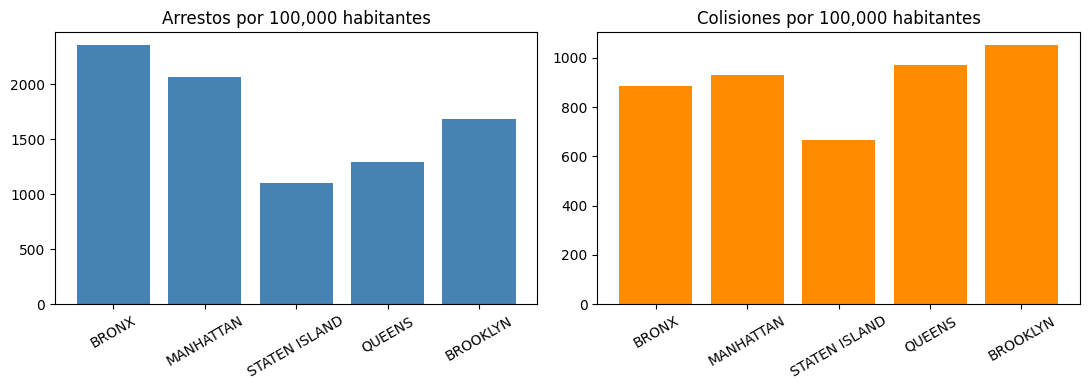
\includegraphics[width=0.92\textwidth]{imagenes/fig_cell_43_1.png}
    \caption{Comparación de tasas estandarizadas de arrestos y colisiones por cada 100,000 habitantes entre los cinco condados.}
    \label{fig:tasas_100k}
\end{figure}

\noindent \textbf{Hallazgo clave de la estandarización:} Mientras que en cifras brutas Brooklyn ocupaba el primer lugar en arrestos ($42,877$), al normalizar por la población estimada de cada condado \textbf{El Bronx pasa a encabezar la tasa de detenciones con $2,354.5$ arrestos por cada $100,000$ habitantes}, seguido de Manhattan ($2,064.1$, influenciado por su alta población flotante) y desplazando a Brooklyn al tercer lugar ($1,687.6$). En contraste, en siniestralidad vial de 2025, \textbf{Brooklyn mantiene el primer lugar tanto en volumen absoluto ($26,712$) como en tasa relativa ($1,051.4$ colisiones por cada $100,000$ habitantes)}, seguido por Queens ($970.3$).

\subsubsection{Verificación de Severidad Vial tras el Filtrado de Integridad (Elemento 8 Depurado)}

Una vez aplicados los filtros F1, F2 y F3 sobre el histórico de colisiones ($2,305,355$ registros limpios), se recalculó la distribución acumulada de heridos y fallecidos por tipo de actor vial (Figura \ref{fig:severidad_colisiones_limpia}). Se verifica la eliminación total de la distorsión detectada en la exploración preliminar: el histórico limpio registra exactamente \textbf{$779,372$ personas heridas} y \textbf{$3,746$ personas fallecidas}. Los ocupantes de vehículos motorizados concentran el mayor volumen de heridos ($552,978$, seguidos de $141,625$ peatones y $68,866$ ciclistas), pero \textbf{los peatones concentran la mayor cantidad de víctimas mortales ($1,847$ fallecidos, equivalentes al $49.3\%$ del total de muertes viales)}, superando a los motoristas ($1,484$) y ciclistas ($273$).

\begin{figure}[H]
    \centering
    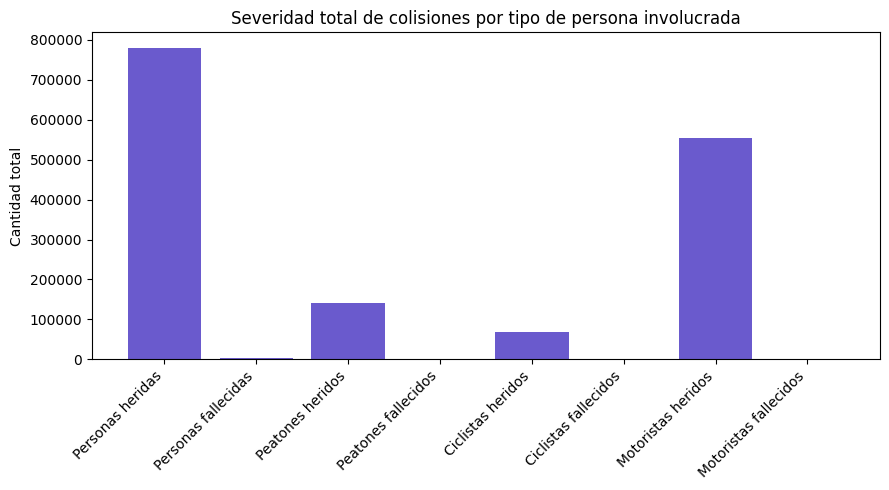
\includegraphics[width=0.78\textwidth]{imagenes/fig_cell_46_1.png}
    \caption{Severidad total acumulada de colisiones por tipo de persona involucrada sobre el conjunto depurado ($2,305,355$ siniestros).}
    \label{fig:severidad_colisiones_limpia}
\end{figure}
